% Options for packages loaded elsewhere
\PassOptionsToPackage{unicode}{hyperref}
\PassOptionsToPackage{hyphens}{url}
%
%\documentclass[
%]{book}
\documentclass[landscape, 20pt]{extreport}
\usepackage{amsmath,amssymb}
\usepackage{lmodern}
\usepackage{iftex}
\ifPDFTeX
  \usepackage[T1]{fontenc}
  \usepackage[utf8]{inputenc}
  \usepackage{textcomp} % provide euro and other symbols
\else % if luatex or xetex
  \usepackage{unicode-math}
  \defaultfontfeatures{Scale=MatchLowercase}
  \defaultfontfeatures[\rmfamily]{Ligatures=TeX,Scale=1}
\fi
% Use upquote if available, for straight quotes in verbatim environments
\IfFileExists{upquote.sty}{\usepackage{upquote}}{}
\IfFileExists{microtype.sty}{% use microtype if available
  \usepackage[]{microtype}
  \UseMicrotypeSet[protrusion]{basicmath} % disable protrusion for tt fonts
}{}
\makeatletter
\@ifundefined{KOMAClassName}{% if non-KOMA class
  \IfFileExists{parskip.sty}{%
    \usepackage{parskip}
  }{% else
    \setlength{\parindent}{0pt}
    \setlength{\parskip}{6pt plus 2pt minus 1pt}}
}{% if KOMA class
  \KOMAoptions{parskip=half}}
\makeatother
\usepackage{xcolor}
\IfFileExists{xurl.sty}{\usepackage{xurl}}{} % add URL line breaks if available
\IfFileExists{bookmark.sty}{\usepackage{bookmark}}{\usepackage{hyperref}}
\hypersetup{
  pdftitle={SCMA329 Practical Mathematical Financial Modeling},
  pdfauthor={Pairote Satiracoo},
  hidelinks,
  pdfcreator={LaTeX via pandoc}}
\urlstyle{same} % disable monospaced font for URLs
\usepackage[margin=1in]{geometry}
\usepackage{longtable,booktabs,array}
\usepackage{calc} % for calculating minipage widths
% Correct order of tables after \paragraph or \subparagraph
\usepackage{etoolbox}
\makeatletter
\patchcmd\longtable{\par}{\if@noskipsec\mbox{}\fi\par}{}{}
\makeatother
% Allow footnotes in longtable head/foot
\IfFileExists{footnotehyper.sty}{\usepackage{footnotehyper}}{\usepackage{footnote}}
\makesavenoteenv{longtable}
\usepackage{graphicx}
\makeatletter
\def\maxwidth{\ifdim\Gin@nat@width>\linewidth\linewidth\else\Gin@nat@width\fi}
\def\maxheight{\ifdim\Gin@nat@height>\textheight\textheight\else\Gin@nat@height\fi}
\makeatother
% Scale images if necessary, so that they will not overflow the page
% margins by default, and it is still possible to overwrite the defaults
% using explicit options in \includegraphics[width, height, ...]{}
\setkeys{Gin}{width=\maxwidth,height=\maxheight,keepaspectratio}
% Set default figure placement to htbp
\makeatletter
\def\fps@figure{htbp}
\makeatother
\setlength{\emergencystretch}{3em} % prevent overfull lines
\providecommand{\tightlist}{%
  \setlength{\itemsep}{0pt}\setlength{\parskip}{0pt}}
\setcounter{secnumdepth}{5}
\usepackage{booktabs}
\usepackage{amsthm}
\usepackage{LectureNoteMacro}
\usepackage{actuarialangle}
\usepackage{bbm}
\usepackage{mathtools}
\makeatletter
\def\thm@space@setup{%
  \thm@preskip=8pt plus 2pt minus 4pt
  \thm@postskip=\thm@preskip
}
\makeatother
\ifLuaTeX
  \usepackage{selnolig}  % disable illegal ligatures
\fi
\usepackage[]{natbib}
\bibliographystyle{apalike}

\title{SCMA329 Practical Mathematical Financial Modeling}
\author{Pairote Satiracoo}
\date{2022-08-14}

\usepackage{amsthm}
\newtheorem{theorem}{Theorem}[chapter]
\newtheorem{lemma}{Lemma}[chapter]
\newtheorem{corollary}{Corollary}[chapter]
\newtheorem{proposition}{Proposition}[chapter]
\newtheorem{conjecture}{Conjecture}[chapter]
\theoremstyle{definition}
\newtheorem{definition}{Definition}[chapter]
\theoremstyle{definition}
\newtheorem{example}{Example}[chapter]
\theoremstyle{definition}
\newtheorem{exercise}{Exercise}[chapter]
\theoremstyle{definition}
\newtheorem{hypothesis}{Hypothesis}[chapter]
\theoremstyle{remark}
\newtheorem*{remark}{Remark}
\newtheorem*{solution}{Solution}
\begin{document}
\maketitle

{
\setcounter{tocdepth}{1}
%\tableofcontents
}
\hypertarget{cashflows-interest-and-the-time-value-of-money}{%
\chapter{Cashflows, Interest and the Time Value of Money}\label{cashflows-interest-and-the-time-value-of-money}}

\hypertarget{introduction-to-financial-modelling}{%
\newpage \section{Introduction to Financial Modelling}\label{introduction-to-financial-modelling}}

A financial model is a financial representation of a real world
financial situation, which is either a mathematical or statistical model
that describes the relationship among the variables of the financial
problem. Here are some types of financial models.

\begin{itemize}
\item
  \textbf{Financial statement model:} The model includes three main
  components including income statement, cash flow statement and
  balance sheet. These are accounting reports issued by a company
  quarterly and annually that are used for decision making and
  performing financial analysis. (see
  \url{https://corporatefinanceinstitute.com/resources/knowledge/accounting/three-financial-statements/})
\item
  \textbf{Project finance models:} The model incorporates two main elements
  of the project including loans and debt repayment. It can be used to
  assess the risk-reward of lending to or investing in a long-term
  project, i.e.~it can be used to tell whether the project has enough
  cash to cover the debt in the long term. (see
  \url{https://www.wallstreetprep.com/knowledge/project-finance-model-structure/})
\item
  \textbf{Discounted cashflow model:} It is the model to value a company
  using the net present value of the business's future cashflows, or
  to estimate the value of an investment based on its future cash
  flows. (see
  \url{https://corporatefinanceinstitute.com/resources/templates/excel-modeling/dcf-model-template/})
\item
  \textbf{Pricing models:} This models the way prices are set within a
  market in order to maximise profits.
\end{itemize}

This chapter covers the basic concepts of calculating interest,
including simple and compound interest, the frequency of compounding,
the effective interest rate and the discount rate, and the present and
future values of a single payment.

\hypertarget{cashflows}{%
\newpage \section{Cashflows}\label{cashflows}}

Cashflows are amounts of money which are received (or income, positive
cashflows) or paid (or outgo, negative cashflows) at particular times.
Those payments arise from a financial transaction, e.g

\begin{itemize}
\item
  a bank account,
\item
  a loan,
\item
  an equity,
\item
  a zero-coupon bond: A bond is a fixed income instrument that
  represents a loan from an investor to a debtor either a government
  or a corporation. A zero-coupon bond is a bond that pays no interest
  during its life.
\item
  a fixed interest security: A fixed-income security is a debt
  instrument such as a bond or debenture that investors use to lend
  money to a company in exchange for interest payments.
\item
  an index-linked security: An index-linked bonds pay interest that is
  tied to an underlying index, such as the consumer price index (CPI).
  Index-linked bonds are issued by governments to mitigate the effects
  of inflation by paying a real return plus accrued inflation.
\item
  an annuity: An annuity is a series of payments made at regular
  intervals, such as equal monthly payments on a mortgage.
\item
  a capital project etc.
\end{itemize}

Cash received represents inflows, income or also called \textbf{positive
cashflows}, while money spent represents outflows, outgo or \textbf{negative
cashflows}. The net cashflow at a given point in time is the difference
between expenses and income.

\newpage \begin{example}
\protect\hypertarget{exm:unlabeled-div-1}{}\label{exm:unlabeled-div-1}

\emph{A series of payments into and out of a bank account is given as
follows:}

\begin{itemize}
\item
  \emph{payments into the account : ฿1000 on 1 January 2014 and ฿100 on 1
  January 2016}
\item
  \emph{payments out of the account : ฿200 on 1 July 2015, ฿300 on 1 July
  2016, and ฿400 on 1 January 2018}
\end{itemize}

\end{example}

In practice, cashflows can be represented by a timeline as can be
illustrated in this example.

\begin{figure}

{\centering 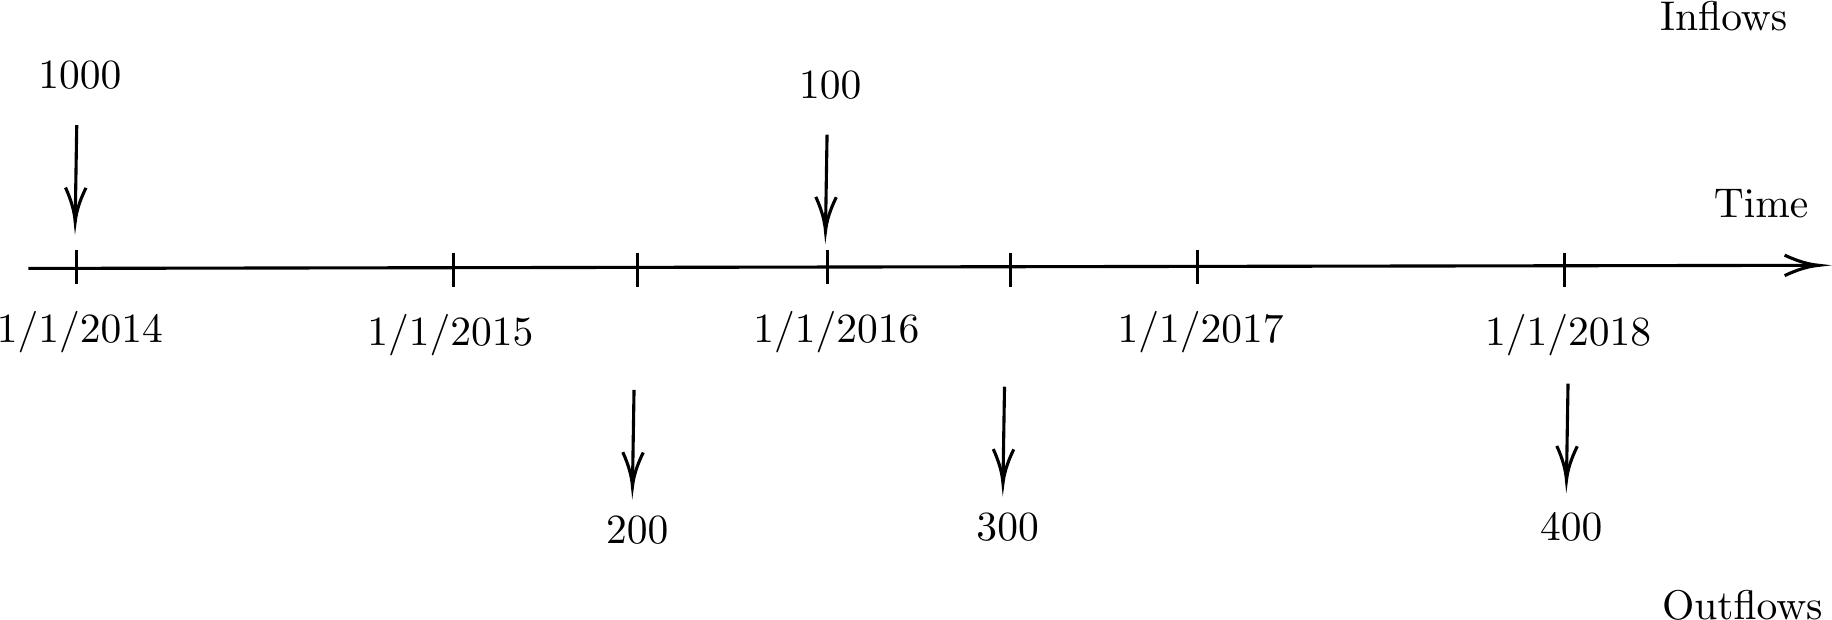
\includegraphics{tikz-ex1-1} 

}

\caption{an example of a timeline}\label{fig:tikz-ex1}
\end{figure}

\hypertarget{interest-and-the-time-value-of-money}{%
\newpage \section{Interest and the Time Value of Money}\label{interest-and-the-time-value-of-money}}

This section introduces the time value of money using the concepts of
compound interest and discounting. The effect of interest rates on the
present value of future cash flows is discussed. The value of distant
cash flows in the present and current cash flows in the future are then
considered.

We illustrate the time value of money by considering the following
examples.

\newpage \begin{example}
\protect\hypertarget{exm:egpv}{}\label{exm:egpv}

\emph{An investor want to make a payment of ฿10000 in 2 years. Suppose that a
bank pays compound interest at 4\% per annum effective. How much should
the initial investment?}

\end{example}

\textbf{Note} The amount we need to invest now (i.e.~the initial investment
in this example) is called the \emph{present value (PV)} or \emph{discounted
value} of the payments.

\textbf{Solution:} The interest for year 1 is

\[ X \cdot 0.04.\] For year 2 the principal is

\[ X + X \cdot 0.04 = X \cdot (1 + 0.04)\] so that the interest for the
year is

\[ X \cdot (1 + 0.04) \cdot 0.04.\]

By the end of 2 years an initial payment of ฿X will have accumulated to:

\[X\cdot (1 + 0.04) + X \cdot (1 + 0.04) \cdot 0.04 =   X  \cdot  1.04^2 = 10000.\]
Hence,

\[X = \frac{10000}{1.04^2} = 9245.56213,\]

\textbf{Note} We refer to the amount to which the capital accumulates with
the addition of interest as \emph{accumulation} or \emph{accumulated value}.

\newpage \begin{example}
\protect\hypertarget{exm:unlabeled-div-2}{}\label{exm:unlabeled-div-2}

\emph{Consider the following arguments}

\begin{itemize}
\item
  \emph{It is obvious that you would prefer to have ฿1100 now than ฿1000
  now.}
\item
  \emph{If we receive and hold ฿1 now, then it is worth more than receiving
  and holding ฿1 at some time in the future? Why is this?}
\item
  \emph{Is it obvious that your would be better off with ฿1100 in 2 years
  than ฿1000 now?}
\end{itemize}

\end{example}

\textbf{Solution:}

For the second argument, this one baht will grow to \(1 + r\) in the first
year, \((1 + r)^2\) in two years, and so on. These amounts are clearly
worth more than receiving and holding ฿1 at the same time in the future.

For the last argument, we need to compare the values of the amounts
**received at different times. To do this, we can look at the today's
values of ฿1100 received in 2 years assuming that we can invest at an
annual interest rate of \(r\) percent.

The present value of this amount \(X\) in year 2 is \[ 1100/(1 + r)^2.\] Assuming \(r = 5\%\), the present value of \(X\) is 997.7324263.

Comparing the values in today's baths, it is better to
have ฿1000 now than to have ฿1100 in 2 years.

\textbf{Notes} From the above example,

\begin{enumerate}
\def\labelenumi{\arabic{enumi}.}
\item
  One can deposit or invest ฿1 now and will receive ฿1 back and a
  reward called \emph{interest} at some point in the future. Because of its
  potential earning power, money in the present is worth more than an
  equal amount in the future. This is a fundamental financial
  principle known as \textbf{the time value of money}.
\item
  At a given point of time, cash has a monetary value, but also has a
  \emph{time value}.
\item
  The amount deposited or invested is called \emph{capital} or \emph{principal}.
\end{enumerate}

\hypertarget{simple-interest}{%
\newpage \subsection{Simple interest}\label{simple-interest}}

Simple interest is a calculation of interest that does not take into
account the effect of compounding. Under simple interest, the amount of interest that accrues over time is proportional to the length of the period.

Suppose an amount \(C\) is deposited in
an account that pays simple interest at the rate of \(i\)\% per annum. Then
after \(n\) years the deposit will have accumulated to
\[C( 1 + i \cdot n).\] Hence, the interest accrued over \(n\) years is
\[\text{Simple Interest}  = C \cdot i \cdot n.\]

\textbf{Note} Auto loans and short-term personal loans are usually simple
interest loans.

\newpage \begin{example}
\protect\hypertarget{exm:unlabeled-div-3}{}\label{exm:unlabeled-div-3}

\emph{An investor deposits ฿10000 in a bank account that pays simple interest
at a rate of 5\% per annum. Calculate}

\begin{enumerate}
\def\labelenumi{\arabic{enumi}.}
\item
  \emph{interest he will earn after the first two years.}
\item
  \emph{interest he will earn after the first three months.}
\end{enumerate}

\end{example}

\textbf{Note} When \(n\) is not an integer, interest is paid on a pro-rate
basis (in proportion).

\textbf{Solution:}

\begin{enumerate}
\def\labelenumi{\arabic{enumi}.}
\item
  At the end of 2 years the interest earned is
  \[10000 \cdot 0.05 \cdot 2 = 1000.\]
\item
  At the end of 3 months the interest earned is
  \[10000 \cdot 0.05 \cdot \frac{3}{12} = 125.\] Alternatively, the
  interest per month is 5\%/12 = 0.4167\% and hence the interest earned
  can be calculated as \[10000 \cdot 0.004167 \cdot 3 = 125.\]
\end{enumerate}

\hypertarget{compound-interest}{%
\newpage \subsection{Compound interest}\label{compound-interest}}

In compound interest, the accumulated amount over a period of time is the capital of the following period. Therefore, a capital of 1 unit at the end of the year increases to \(1 + i\) units, which becomes the capital for the following year.

For year 2, the principal is \(1 + i\) and the interest for the year is
\(( 1 + i ) \cdot i\). By the end of 2 years, an initial payment of 1 will have accumuulated to
\[ (1+i) + ( 1 + i ) \cdot i = (1+i)^2.\]

As this progression continues, the accumulated amount of \(X\) units at the end of year \(n\) becomes
\[ X\cdot(1 + i)^n. \]

\theNote In this case, we can take money out and reinvest it as new capital illustrated in the timeline.

\begin{figure}

{\centering 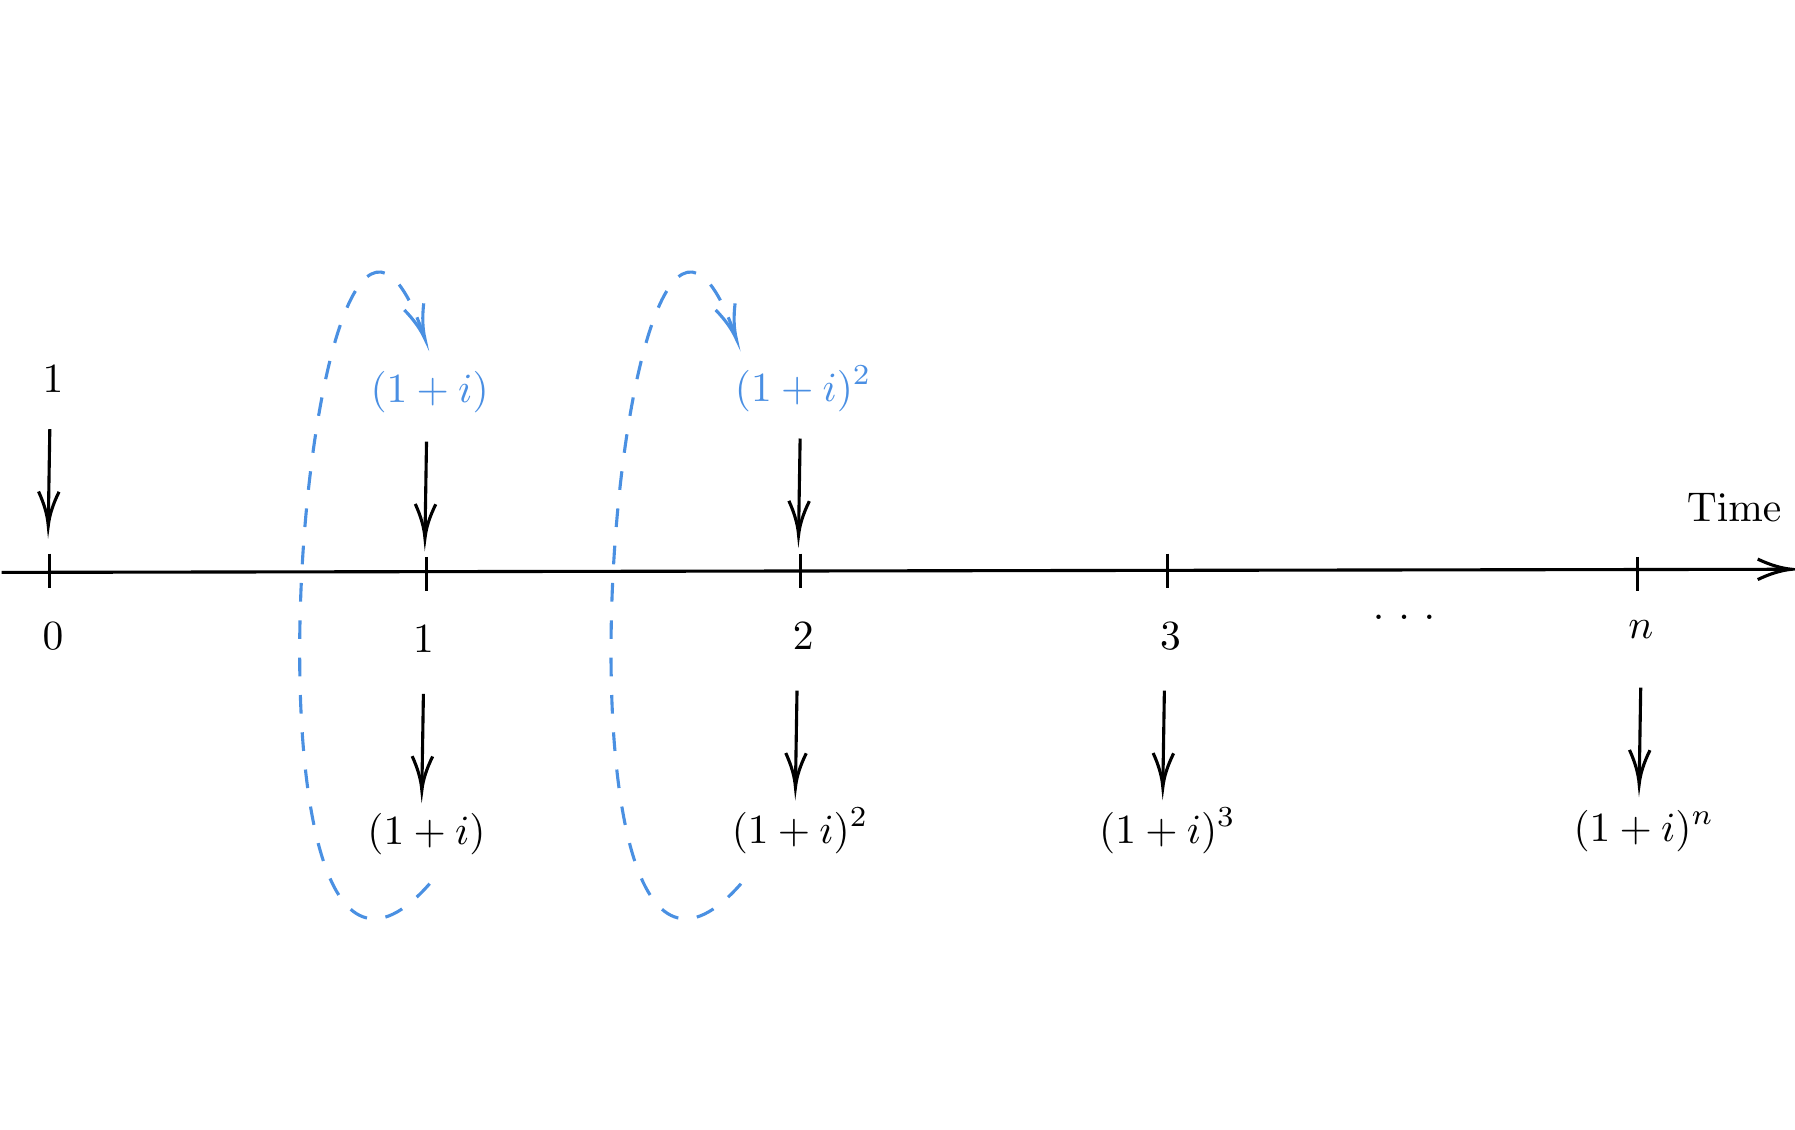
\includegraphics{tikz-ex2-1} 

}

\caption{a timeline of compounding interest}\label{fig:tikz-ex2}
\end{figure}

\begin{exercise}
\protect\hypertarget{exr:unlabeled-div-4}{}\label{exr:unlabeled-div-4}

(Excel) Use Excel to create a table showing the accumulated amounts at the end of each year for 15 years for a principal of ฿100 under the simple interest approach and the compound interest approach with \(r = 6\%\) for both cases.
Discuss the results obtained (How long does it take to double the investment? How much will the principal grow over a 15-year period?)

\end{exercise}

The effect of compounding is to increase the total amount of accumulation. The effect is greater when the interest rate is high. This example shows two examples of the accumulated amount of ฿100 under the simple interest approach and the compound interest approach. As can be seen, the compound interest method makes the principle increase much faster than the simple interest method when the interest rate is high.

\hypertarget{frequency-of-compounding}{%
\newpage \section{Frequency of Compounding}\label{frequency-of-compounding}}

Even though the interest rate is typically expressed in annual terms, an investment's interest is frequently paid more frequently than once per year. For example, a savings account may offer an interest rate of 4\% per year, credited quarterly. This interest rate is usually referred to as \textbf{nominal rate of interest}, i.e., 4\% due four times per year.

We will see that the frequency of interest payments, also known as the frequency of compounding, has a significant impact on the total amount accrued and the interest collected. Consequently, it is crucial to precisely specify the rate of interest.

We use \(i^{(m)}\) to represent the nominal rate of interest payable \(m\) times a year in order to underline the significance of the frequency of compounding. Therefore, \(m\) is the
frequency of compounding per year and \(1/m\) year is the \textbf{compounding period} or \textbf{conversion period}.

\textbf{Note} The nominal rate of interest payable \(m\) times per period is also known as the rate of interest convertible \(m\)thly or compounded \(m\)thly.

\newpage \begin{example}
\protect\hypertarget{exm:unlabeled-div-5}{}\label{exm:unlabeled-div-5}

Calculate the accumulated value in 1 year of a deposit of ฿100 in a saving account that earns interest at 10\% payable quarterly.

\end{example}

\textbf{Solution:} In this example, the nominal rate of interest of \(i^{(4)} = 10\%\) p.a. convertible
quarterly means an interest rate of 10\%/4 = 2.5\% per quarter. In this case, the interest rate of 2.5\% is called \emph{effective interest}. The effective interest rate of \(i\) per unit of time (which may be month, quarter, etc.) is the amount of interest received at the end of a unit of time per ฿1 invested at the beginning of that unit.

Therefore, the nominal interest rate \(i^{(4)} = 10\%\) is equivalent to an
\emph{effective interest rate} of \(2.5\%\) per quarter.
The accumulated value in
1 year is \(100 (1 + \frac{10\%}{4})^4 = 100 (1 + 2.5\%)^4 = 110.3813\).

Note that after compound interest is
taken into account, the interest income of an investor at the quarterly
convertible nominal interest rate of 10\% p.a. is 10.3813 (or 10.3813\%.p.a. effective)

\newpage \begin{example}
\protect\hypertarget{exm:unlabeled-div-6}{}\label{exm:unlabeled-div-6}

\emph{At a rate of 12\% p.a. effective, draw a timeline to show cashflows if
฿100 is invested at the start of the year.}

\end{example}

\textbf{Solution:} The accumulated value of ฿100 at the end of the year is
\(100 (1 + 12\%) = 112\).

\newpage \begin{example}
\protect\hypertarget{exm:unlabeled-div-7}{}\label{exm:unlabeled-div-7}

\emph{At a rate of 12\% p.a. compounding quarterly, draw a time line to show
cashflows if ฿100 is invested at the start of the year.}

\end{example}

\textbf{Solution:} The nominal interest rate \(i^{(4)} = 12\%\) is equivalent
to an effective interest rate of \(3\%\) per quarter. The accumulated
value in 1 year is \(100 (1 + 3\%)^4 = 112.55\). After compound interest
is taken into account, the interest income of an investor at the
quarterly convertible nominal interest rate of 10\% p.a. is 12.55 (or
12.55\%. p.a. effective)

\textbf{Note} \(i^{(m)}\) is a nominal rate of interest which is equivalent to \(i^{(m)}/m\) applied for
each \(m\)th of a period. The interest is paid \(m\) times per measurement period.

The value at time \(n\) can be considered as the \textbf{annuity} with a cashflow of \(i^{(m)}/m\) per period for \(n\) years together with the capital at time \(n\) as shown in the following figure.
Therefore, the accumulated value in 1 year can also be calculated as \(100( 1 + 0.03 s_{\angl{4}}^{3\%})\). The concept of annuity will be discussed in the subsequent section.

\begin{figure}

{\centering 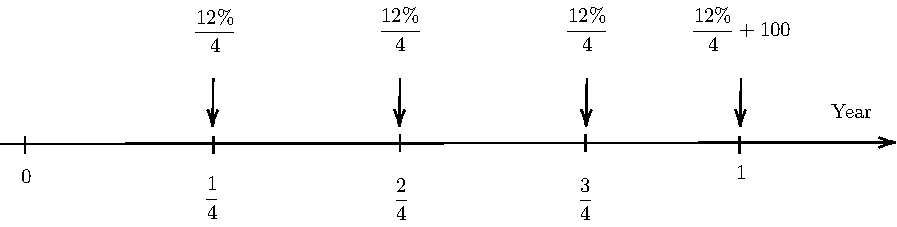
\includegraphics{tikz-ex5-1} 

}

\caption{Frequency of Compouding vs Annuity}\label{fig:tikz-ex5}
\end{figure}

In general, we have

\begin{figure}

{\centering 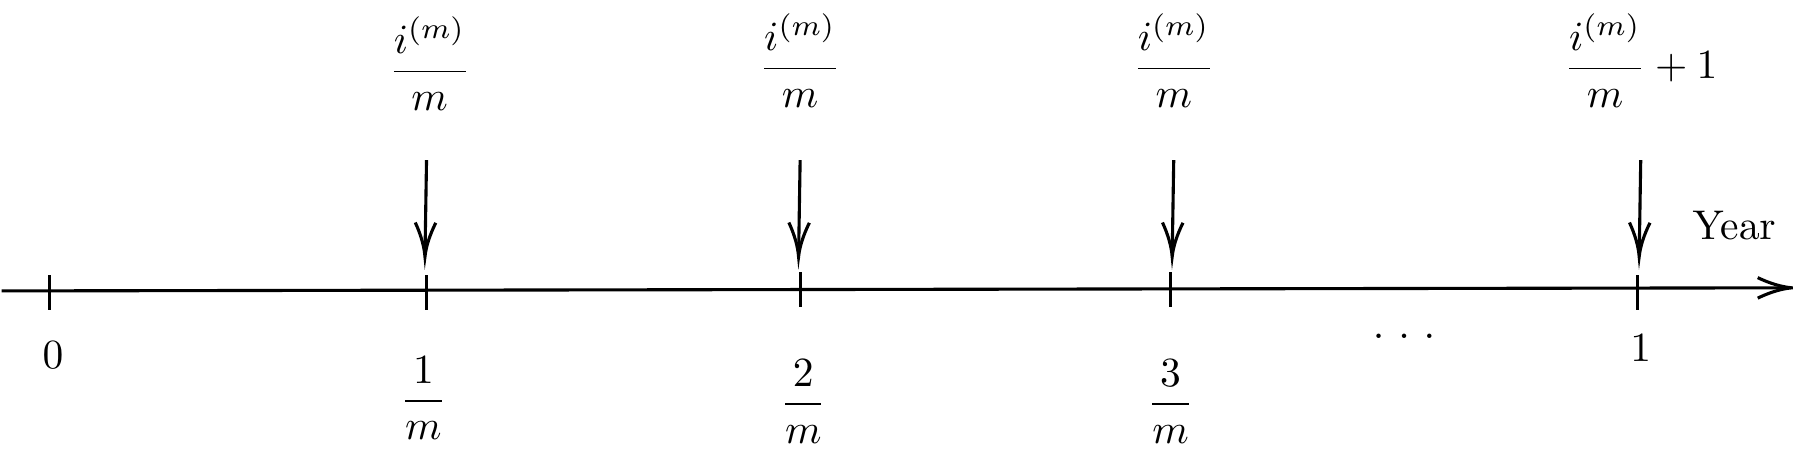
\includegraphics{tikz-ex4-1} 

}

\caption{Frequency of Compouding vs Annuity}\label{fig:tikz-ex4}
\end{figure}

\hypertarget{effective-rate-of-interest}{%
\newpage \subsection{Effective rate of interest}\label{effective-rate-of-interest}}

The compounding frequency affects the accumulated amount. As a result, it may be inaccurate to compare two investment strategies only based on their nominal rates of return without also taking into account their frequency of compounding. It is necessary to compare different investment strategies on an equal basis. The measure known as the \textbf{effective interest rate} is often used for this purpose.

The effective rate of interest of \(i\) per time unit is the amount of
interest received at the end of one time unit per ฿1 invested at the
start of that time unit.

\newpage \begin{example}
\protect\hypertarget{exm:unlabeled-div-8}{}\label{exm:unlabeled-div-8}

\emph{An investor invests ฿1 at 7.5\% p.a. (per annum) effective. Then}
\(i = 0.075\). Calculate the value of investment after one year.

\end{example}

\textbf{Solution:} The value of investment after one year at this rate is
\[1 \times ( 1 + 0.075) = 1.075.\]
In particular, the amount of
interest received at the end of the year per ฿1 invested is 0.075.

\newpage \begin{example}
\protect\hypertarget{exm:unlabeled-div-9}{}\label{exm:unlabeled-div-9}

\emph{An investor invests ฿1000 at 5.25\% per half-year effective. Then}
\(i = 0.0525\). Calculate the value of investment after half a year.

\end{example}

\textbf{Solution:} The value of investment after half year at this rate is
\[1000 \times ( 1 + 0.0525) = 1052.5.\]
Again, the amount ofinterest received at the end of the quarter of ฿1 invested is 0.0525.

\textbf{Note} The time unit is an \textbf{essential part of the definition}.

\newpage \begin{example}
\protect\hypertarget{exm:unlabeled-div-10}{}\label{exm:unlabeled-div-10}

\emph{An investor invests ฿1 at effective rate} \(i\)\% per time unit for \(n\)
time units. Calculate the value of investment after two, three,
\(\ldots\), \(n\) time units.

\end{example}

\textbf{Note} Here we assume that we can take money out and reinvest it as
new capital (see the timeline).

\begin{center}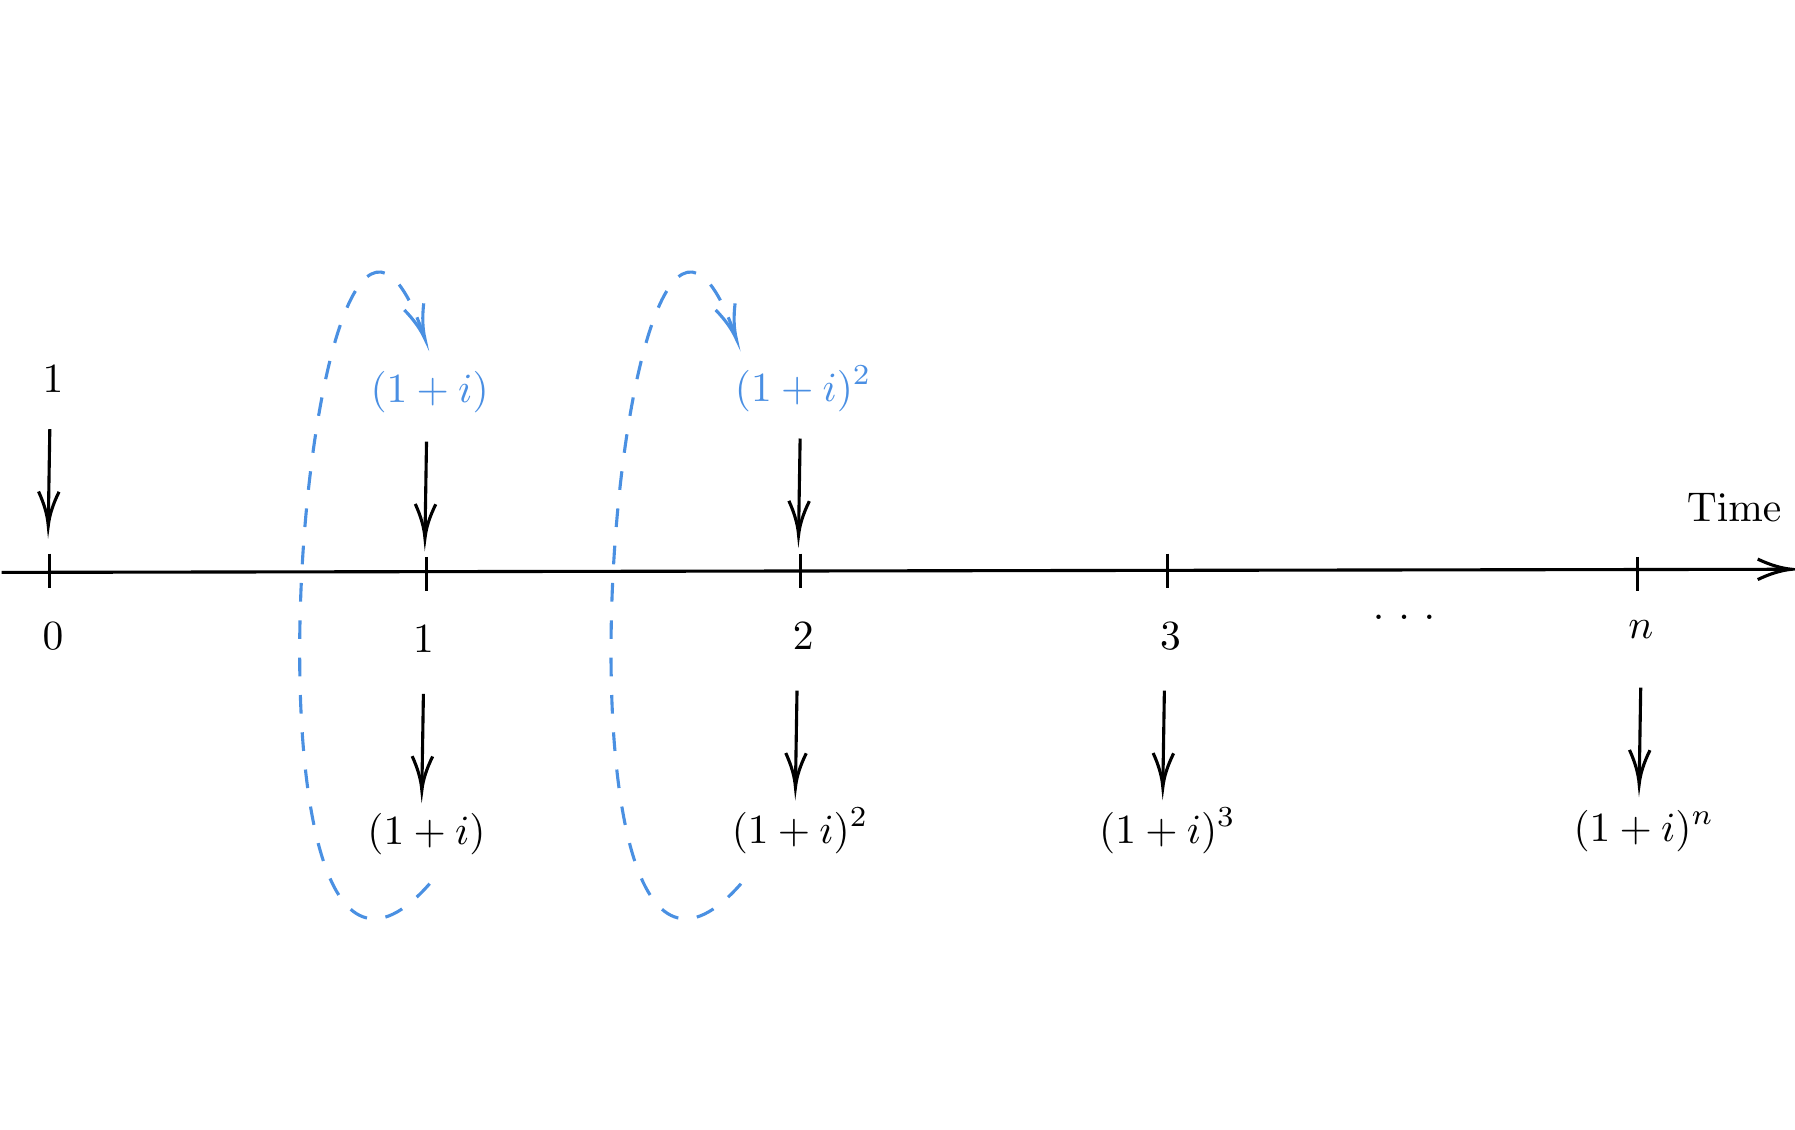
\includegraphics{tikz-ex6-1} \end{center}

\newpage \begin{example}
\protect\hypertarget{exm:unlabeled-div-11}{}\label{exm:unlabeled-div-11}

\emph{An investor invests ฿200 at} \(3\)\% pa effective. What will be the
deposit have accumulated to after 5 years.

\end{example}

\textbf{Solution:} The deposit accumulates to
\(200 \cdot (1.03)^5 = 231.854815\) after 5 years.

\newpage \begin{example}
\protect\hypertarget{exm:unlabeled-div-12}{}\label{exm:unlabeled-div-12}

Consider the following problems.

\begin{enumerate}
\def\labelenumi{\arabic{enumi}.}
\item
  \emph{An investor invests ฿500 at} \(2.75\)\% per quarter effective. What
  will be the deposit have accumulated to after 9 months.
\item
  \emph{An investor invests ฿2000 at} \(6\)\% per half-year effective. What
  will be the deposit have accumulated to after 2 years.
\end{enumerate}

\end{example}

\textbf{Solution:}

\begin{enumerate}
\def\labelenumi{\arabic{enumi}.}
\item
  Accumulating the 500 for 9 months at this rate gives
  \[500 \cdot (1.0275)^3 = 542.394773.\]
\item
  After 2 years the accumulation is
  \[2000 \cdot (1.06)^4 = 2524.95392.\]
\end{enumerate}

\textbf{Notes}

\begin{enumerate}
\def\labelenumi{\arabic{enumi}.}
\item
  The model under the effective rate of interest condition is a
  model of \emph{compound interest}, where interest is earned on interest
  previously earned. Unless state otherwise, we shall assume that \(i\) is
  the compound interest rate.
\item
  In practice, it is easier to work with the effective rate of
  interest which is defined in a suitable time unit.
\end{enumerate}

The following formula can be used to convert between the effective rate
\(i\) p.a. and the nominal rate \(i^{(m)}\) p.a.:
\[( 1 + i) = \left( 1 + \frac{i^{(m)}}{m}\right)^m.\]

\newpage \begin{example}
\protect\hypertarget{exm:unlabeled-div-13}{}\label{exm:unlabeled-div-13}

Consider the following problems.

\begin{enumerate}
\def\labelenumi{\arabic{enumi}.}
\item
  \emph{Express a nominal annual interest rate of 9\% convertible
  half-yearly as a monthly effective interest.}
\item
  \emph{Express a two-monthly effective interest of 3\% as a nominal annual
  interest rate convertible two-monthly.}
\end{enumerate}

\end{example}

\textbf{Solution:}

\begin{enumerate}
\def\labelenumi{\arabic{enumi}.}
\item
  The effective rate \(i\)\% p.a. is \[i = ( 1 + \frac{0.09}{2})^2 - 1.\]
  Hence the monthly effective rate is
  \(j = (1 + i)^{1/12} - 1 = ( 1 + \frac{0.09}{2})^{2/12} - 1 = 0.007363\).
\item
  A nominal annual interest rate convertible two-monthly is
  \(6 \cdot 3\% = 18\%\).
\end{enumerate}

\newpage \begin{example}
\protect\hypertarget{exm:unlabeled-div-14}{}\label{exm:unlabeled-div-14}

\emph{Express each of the following effective rates per annum as a nominal
rate, and vice versa.}

\begin{longtable}[]{@{}ll@{}}
\toprule
\textbf{\emph{Effective Rate}} & \textbf{\emph{Nominal Rate}} \\
\midrule
\endhead
\(i\) = 0.04 & \(i^{(4)} = 0.039412\) \\
\(i\) = 0.10 & \(i^{(12)} = 0.095690\) \\
\(i\) = 0.06152 & \(i^{(2)} = 0.06\) \\
\(i\) = 0.126825 & \(i^{(12)} = 0.12\) \\
\bottomrule
\end{longtable}

\end{example}

\hypertarget{compounding-over-any-number-of-time-units}{%
\newpage \subsection{Compounding over any number of time units}\label{compounding-over-any-number-of-time-units}}

Suppose an amount ฿1 is invested at the rate of \(i\)\% per time unit. At
time \(t\) the accumulation is \((1 + i)^t\).

\newpage \begin{example}
\protect\hypertarget{exm:unlabeled-div-15}{}\label{exm:unlabeled-div-15}

\begin{enumerate}
\def\labelenumi{\arabic{enumi}.}
\item
  \emph{An investor invests ฿4000 at} \(8.5\)\% per quarter effective. What
  will be the deposit have accumulated to after 1 month.
\item
  \emph{An investor invests ฿800 at} \(6\)\% per half-year effective. What
  will be the deposit have accumulated to after 2.6 years.
\end{enumerate}

\end{example}

\textbf{Solution:}

\begin{enumerate}
\def\labelenumi{\arabic{enumi}.}
\item
  The accumulation after 1 month is
  \(4000 \cdot 1.085^{1/3} = 4110.265768.\)
\item
  The accumulation after 2.6 years is
  \(800 \cdot 1.06^{5.2} = 1083.129754.\)
\end{enumerate}

\begin{exercise}
\protect\hypertarget{exr:unlabeled-div-16}{}\label{exr:unlabeled-div-16}

(Excel) Use Excel to create a table showing the accumulated amounts after 1 year under several different compounding frequencies (yearly, quarterly, monthly, daily) for a principal of ฿100 under with nominal rate of \(r = 4\%\) per annum.

Discuss the results obtained. What happens if the compounding is made over infinitely small intervals (i.e.~as \(m \rightarrow \infty\))?

\end{exercise}

\hypertarget{changing-the-time-period-of-the-effective-rates-of-interest}{%
\newpage \subsection{Changing the time period of the effective rates of interest}\label{changing-the-time-period-of-the-effective-rates-of-interest}}

It is often very useful to change the effective rate of interest per
time period to another. For example, if the effective rate of interest
is defined per annum but cashflows occur monthly.

Let \(i\) be the effective rate of interest per \(t_i\) years (which can be
any positive number, for e.g.~\(t_i = 1/2\)). Here \(t_i\) years can be
regarded as one time unit. Let \(j\) be the effective rate of interest per
\(t_j\) years.

\newpage \begin{example}
\protect\hypertarget{exm:unlabeled-div-17}{}\label{exm:unlabeled-div-17}

\emph{Find the condition under which the two effective rates of interest} \(i\)
and \(j\) are equivalent.

\end{example}

\textbf{Solution:} Suppose we invest 1 for one year. Then at the end of the
year under each rate of interest, we will have
\[(1+i)^{1/t_i} \text{ and } (1+j)^{1/t_j}.\] Two rates of interest are
equivalent if the given amount of principal invested for the same length
of time produces the same accumulated value, i.e.
\[(1+i)^{1/t_i} = (1+j)^{1/t_j}.\] Solving the equation for \(j\) yields
\[j = (1+i)^{t_j/t_i} - 1.\]

\newpage \begin{example}
\protect\hypertarget{exm:unlabeled-div-18}{}\label{exm:unlabeled-div-18}

\begin{enumerate}
\def\labelenumi{\arabic{enumi}.}
\item
  \emph{If the effective rate of interest is 6\% per annum, what is the
  effective rate of interest per half-year?}
\item
  \emph{If the effective rate of interest is 12\% per two-years effective,
  what is the effective rate of interest per quarter-year?}
\item
  \emph{If the effective rate of interest is 2\% per month effective, what
  is the effective rate of interest per 1.5-years?}
\end{enumerate}

\end{example}

\textbf{Solution:}

\begin{enumerate}
\def\labelenumi{\arabic{enumi}.}
\item
  \(i = 6\%\) p.a. Then
  \[j = (1.06)^{1/2} -1 = 0.029563 \text{ per half-year}.\]
\item
  \(i = 12\%\) per two-years. Then
  \[j = (1.12)^{1/(2\times4)} -1 = 0.0142669 \text{ per quarter-year}.\]
\item
  \(i = 2\%\) per month. Then
  \[j = (1.02)^{1.5/(1/12)} -1 = 0.428246 \text{ per 1.5-years}.\]
\end{enumerate}

\hypertarget{non-constant-interest-rates}{%
\newpage \subsection{Non-constant interest rates}\label{non-constant-interest-rates}}

The effective rate may not be the same during every time period. We
shall assume that the rates in every future time periods are known in
advance.

\newpage \begin{example}
\protect\hypertarget{exm:unlabeled-div-19}{}\label{exm:unlabeled-div-19}

\emph{The effective rate of interest per annum was 4\% during 2015, 4.5\%
during 2016 and 5\% during 2017. Calculate the accumulation of ฿200
invested on}

\begin{enumerate}
\def\labelenumi{\arabic{enumi}.}
\item
  \emph{01/01/2015 for 3 years}
\item
  \emph{01/07/2015 for 2 years}
\item
  \emph{01/04/2016 for 1.5 years}
\end{enumerate}

\end{example}

\textbf{Solution:}

\begin{enumerate}
\def\labelenumi{\arabic{enumi}.}
\item
  Accumulating the ฿200 for the first year at the rate of 4\% p.a.
  gives \[200 \cdot 1.04.\] The accumulated value was then invested at
  the rate of 4.5\% p.a. for another year, and its value at after 2
  years was \[200 \cdot 1.04 \cdot 1.045.\] At the rate of 5\% in the
  final year, the value after 3 years was
  \[200 \cdot 1.04 \cdot 1.045 \cdot 1.05 = 228.228.\]
\item
  The accumulation is
  \[200 \cdot 1.04^{1/2} \cdot 1.045 \cdot 1.05^{1/2} = 218.4025.\]
\item
  The accumulation is
  \[200 \cdot 1.045^{9/12} \cdot 1.05^{3/4} = 214.416986.\]
\end{enumerate}

\hypertarget{accumulation-factors}{%
\newpage \subsection{Accumulation factors}\label{accumulation-factors}}

Let \(i\) be the effective rate of interest per one time unit and \(s < t\).
We define

\begin{itemize}
\item
  the accumulation factor per one time unit \[A(0,1) = (1 + i).\]
\item
  the accumulation factor per \(t\) time units \[A(0,t) = (1 + i)^t.\]
\item
  the accumulation factor at time \(t\) of 1 unit invested at time \(s\)
  \[A(s,t).\]
\end{itemize}

\newpage \begin{example}
\protect\hypertarget{exm:unlabeled-div-20}{}\label{exm:unlabeled-div-20}

\emph{The effective rate of interest per annum was 6\% during 2015, 8\% during
2016 and 10\% during 2017. Calculate the following accumulation factors.}

\begin{enumerate}
\def\labelenumi{\arabic{enumi}.}
\item
  \(A(01/01/15, 01/01/18),\) i.e.~the accumulation at 01/01/18 of an
  investent of 1 at 01/01/15
\item
  \(A(01/07/15, 01/07/17)\)
\item
  \(A(01/04/16, 01/10/17)\)
\end{enumerate}

\end{example}

\textbf{Solution:}

\begin{enumerate}
\def\labelenumi{\arabic{enumi}.}
\item
  \(A(01/01/15, 01/01/18) = (1.06)(1.08)(1.1) = 1.25928\)
\item
  \(A(01/07/15, 01/07/17) = (1.06)^{1/2}(1.08)(1.1)^{1/2} = 1.166200\)
\item
  \(A(01/04/16, 01/10/17) = (1.08)^{3/4}(1.1)^{3/4} = 1.137922\)
\end{enumerate}

\hypertarget{present-values-and-discount-factors}{%
\newpage \subsection{Present values and discount factors}\label{present-values-and-discount-factors}}

Recall from Example \ref{exm:egpv} that the amount
\(\displaystyle{\frac{10000}{1.04^2}}\) we need to invest now to obtain
฿10000 in two years is called the \emph{present value (PV)} or \emph{discounted
value} of the payments.

We define the discount factor \(v\) per annum, at rate \(i\) p.a. effective
to be the present value of a payment of 1 due in 1 year?s time, i.e.
\[v = \frac{1}{1+i}.\]

\newpage \begin{example}
\protect\hypertarget{exm:unlabeled-div-21}{}\label{exm:unlabeled-div-21}

\emph{Calculate the present of ฿25000 due in 3 years at an effective rate of
interest of 6\% per annum.}

\end{example}

\textbf{Solution:} The present value is
\[25000 \cdot \frac{1}{1.06^3} = 20990.482076.\] It is the discounted
value of 25000 due in 3 years.

\newpage \begin{example}
\protect\hypertarget{exm:unlabeled-div-22}{}\label{exm:unlabeled-div-22}

\emph{How much should we invest now to meet a liability of ฿50000 in 5 years
at an effective rate of interest of 3\% per half-year.}

\end{example}

\textbf{Solution:} The amount we need to invest now to meet the future
liability of 50000 in 5 years is the present value
\[50000 \cdot \frac{1}{1.03^{10}} = 37204.695745.\]

\textbf{Note} It follows that the \(PV\) of ฿1 in \(t\) time units at \(i\)
effective rate of interest per time unit is
\[PV = \frac{1}{(1+i)^t} = v^t.\]

\newpage \begin{example}
\protect\hypertarget{exm:unlabeled-div-23}{}\label{exm:unlabeled-div-23}

\emph{Given the discount factor per year} \(v = 0.9\), calculate

\begin{enumerate}
\def\labelenumi{\arabic{enumi}.}
\item
  \emph{the effective rate of interest per year.}
\item
  \emph{the equivalent discount factor per half-year.}
\end{enumerate}

\end{example}

\textbf{Solution:}

\begin{enumerate}
\def\labelenumi{\arabic{enumi}.}
\item
  From \(\displaystyle{ v= \frac{1}{1+i} = 0.9}\), solving the equation
  for \(i\) gives \[i = \frac{1}{v} - 1 = 0.111111 \text{ per year}.\]
\item
  Let \(j\) be the effective rate of interest per half-year. Then
  \[j = (1+ i)^{1/2} -1 = 0.054093.\] Then, the discount factor per
  half-year is \[v = \frac{1}{1+j} = \frac{1}{1.054093} = 0.948683.\]
\end{enumerate}

Similarly, we define

\begin{itemize}
\item
  the discount factor per one time unit \[V(0,1) = 1/(1 + i).\]
\item
  the discount factor per \(t\) time units \[V(0,t) = 1/(1 + i)^t.\]
\item
  for \(s < t\), the discount factor at time \(s\) of 1 unit receivable at
  time \(t\) \[V(s,t) =  (1 + i)^{s - t}.\]
\end{itemize}

\textbf{Notes}

\begin{enumerate}
\def\labelenumi{\arabic{enumi}.}
\item
  \(V(s,t) = A(s,t)^{-1}\)
\item
  For \(r < s < t\), the following holds:

  \begin{itemize}
  \item
    \(A(r,t) = A(r,s) A(s,t)\)
  \item
    \(V(r,t) = V(r,s) V(s,t)\)
  \end{itemize}
\end{enumerate}


\end{document}
